\documentclass[12pt,a4paper]{article}

% Packages
\usepackage[utf8]{inputenc}
\usepackage{amsmath, amssymb}
\usepackage[a4paper,
  top=1in,
  bottom=1in,
  left=1.25in,
  right=1in]{geometry}
\usepackage{graphicx}
\usepackage{hyperref}
\usepackage{setspace}
\usepackage{titlesec}

\begin{document}

% Title Page
\begin{titlepage}
    \thispagestyle{empty}
    \centering
    \vspace*{\fill} % vertical centering

    % Title (split manually for readability)
    {\Huge \textbf{On the Proximity of Cosmic}}\\[0.2cm]
    {\Huge \textbf{Mass\textendash{}Radius Ratios to}}\\[0.4cm]
    {\Huge \textbf{Black Hole Limits}}\\[0.5cm] % Use -- for en-dash, --- for em-dash

    % Author
    {\LARGE Vinayak Ghai}\\[0.5cm]

    % Subtitle / placeholder
    {\Large Independent Research Project}\\[1cm]

    % Date
    {\Large \today}
    \vspace*{\fill}
\end{titlepage}

\newpage

% Abstract
\begin{abstract}

This study examines how the sizes and masses of cosmic objects—such as stars and planets—relate to the extreme limits that could cause them to collapse into black holes. Black holes are characterized by a critical boundary known as the Schwarzschild radius, beyond which \textbf{gravity} becomes so strong that nothing, not even light, can escape. A natural question arises as to whether these black-hole limits can provide insight into ordinary cosmic objects that exist far from such extreme conditions.

To investigate this, we first apply simplified Newtonian physics, typically introduced at the high-school level. While this approach is mathematically straightforward, it can yield misleading results because it does not fully incorporate the effects predicted by Einstein’s theory of relativity. Relativistic effects become significant when \textbf{gravity} is exceptionally strong or when matter reaches extreme densities.

We then adopt a more rigorous, calculus-based framework that accounts for gravitational effects with greater accuracy. This method produces results that align more closely with relativistic expectations for massive stars and black-hole formation.

Overall, this work highlights the interplay between classical physics and relativity in determining the physical limits of cosmic objects. It clarifies the distinction between ordinary stellar structures and the extreme conditions required for black-hole collapse, offering a clearer perspective on how \textbf{gravity} governs structure and stability across the universe.

\end{abstract}

\newpage

% Sections
\section{Introduction}

\subsection{Background and Motivation}

The Schwarzschild radius emerges naturally in general relativity as a critical scale associated with gravitational collapse. It defines the radius at which the escape velocity from a spherically symmetric mass equals the speed of light, marking the formation of an event horizon. This simple mass-radius relationship is often presented as a clear boundary between ordinary astrophysical objects and black holes.
\begin{equation}
r_s = \frac{2GM}{c^2}
\end{equation}
where $G$ is the gravitational constant, $M$ is the mass of the object, and $c$ is the speed of light. This simple mass-radius relationship is often presented as a clear boundary between ordinary astrophysical objects and black holes.

The apparent simplicity of this criterion makes it tempting to apply it broadly. In particular, expressing the Schwarzschild condition as an inequality involving mass and radius suggests that one might compare ordinary cosmic objects—such as stars or planets—against black hole limits in a direct and quantitative way. Initially, this motivates the idea that meaningful physical insight could be obtained by examining how close such objects come to satisfying this condition.

However, this intuition raises an important question: does mathematical proximity to the Schwarzschild limit necessarily imply physical relevance, or does such reasoning obscure deeper constraints imposed by gravitational theory?

\subsection{Limitations of Naive Schwarzschild Arguments}

The Schwarzschild radius is derived under assumptions such as spherical symmetry, vacuum exterior, and full general relativity. Ignoring these assumptions can produce arguments that are mathematically correct but physically misleading.

In Newtonian terms, the escape velocity from an object is
\begin{equation}
v_\text{esc} = \sqrt{\frac{2GM}{R}},
\end{equation}
and setting $v_\text{esc} = c$ formally gives
\begin{equation}
R = \frac{2GM}{c^2} = r_s,
\end{equation}
explaining the intuitive, classical motivation. However, this neglects relativistic effects, internal pressure, and spacetime curvature, making collapse physically impossible for ordinary objects. 

This tension between mathematical validity and physical meaning motivates the present study, which examines the limits of applying Schwarzschild-based criteria.

\subsection{Scope and Contributions of This Work}

This work investigates the conditions under which Schwarzschild-based mass-radius comparisons retain physical meaning and identifies regimes where such comparisons break down. While the Schwarzschild radius provides a precise boundary for black hole formation, its application to ordinary stars and planets can be misleading when naive Newtonian intuition is applied.

For example, consider a neutron star with mass $M \sim 2 M_\odot$ and radius $R \sim 12~\mathrm{km}$. Using the Newtonian escape velocity formula,
\[
v_\text{esc} = \sqrt{\frac{2GM}{R}} \approx 0.6\,c,
\]
one might conclude that this object is dangerously close to becoming a black hole. However, fully relativistic models show that the internal pressure and equation of state prevent collapse, illustrating the gap between mathematical suggestion and physical reality.

\begin{figure}[ht!]
    \centering
    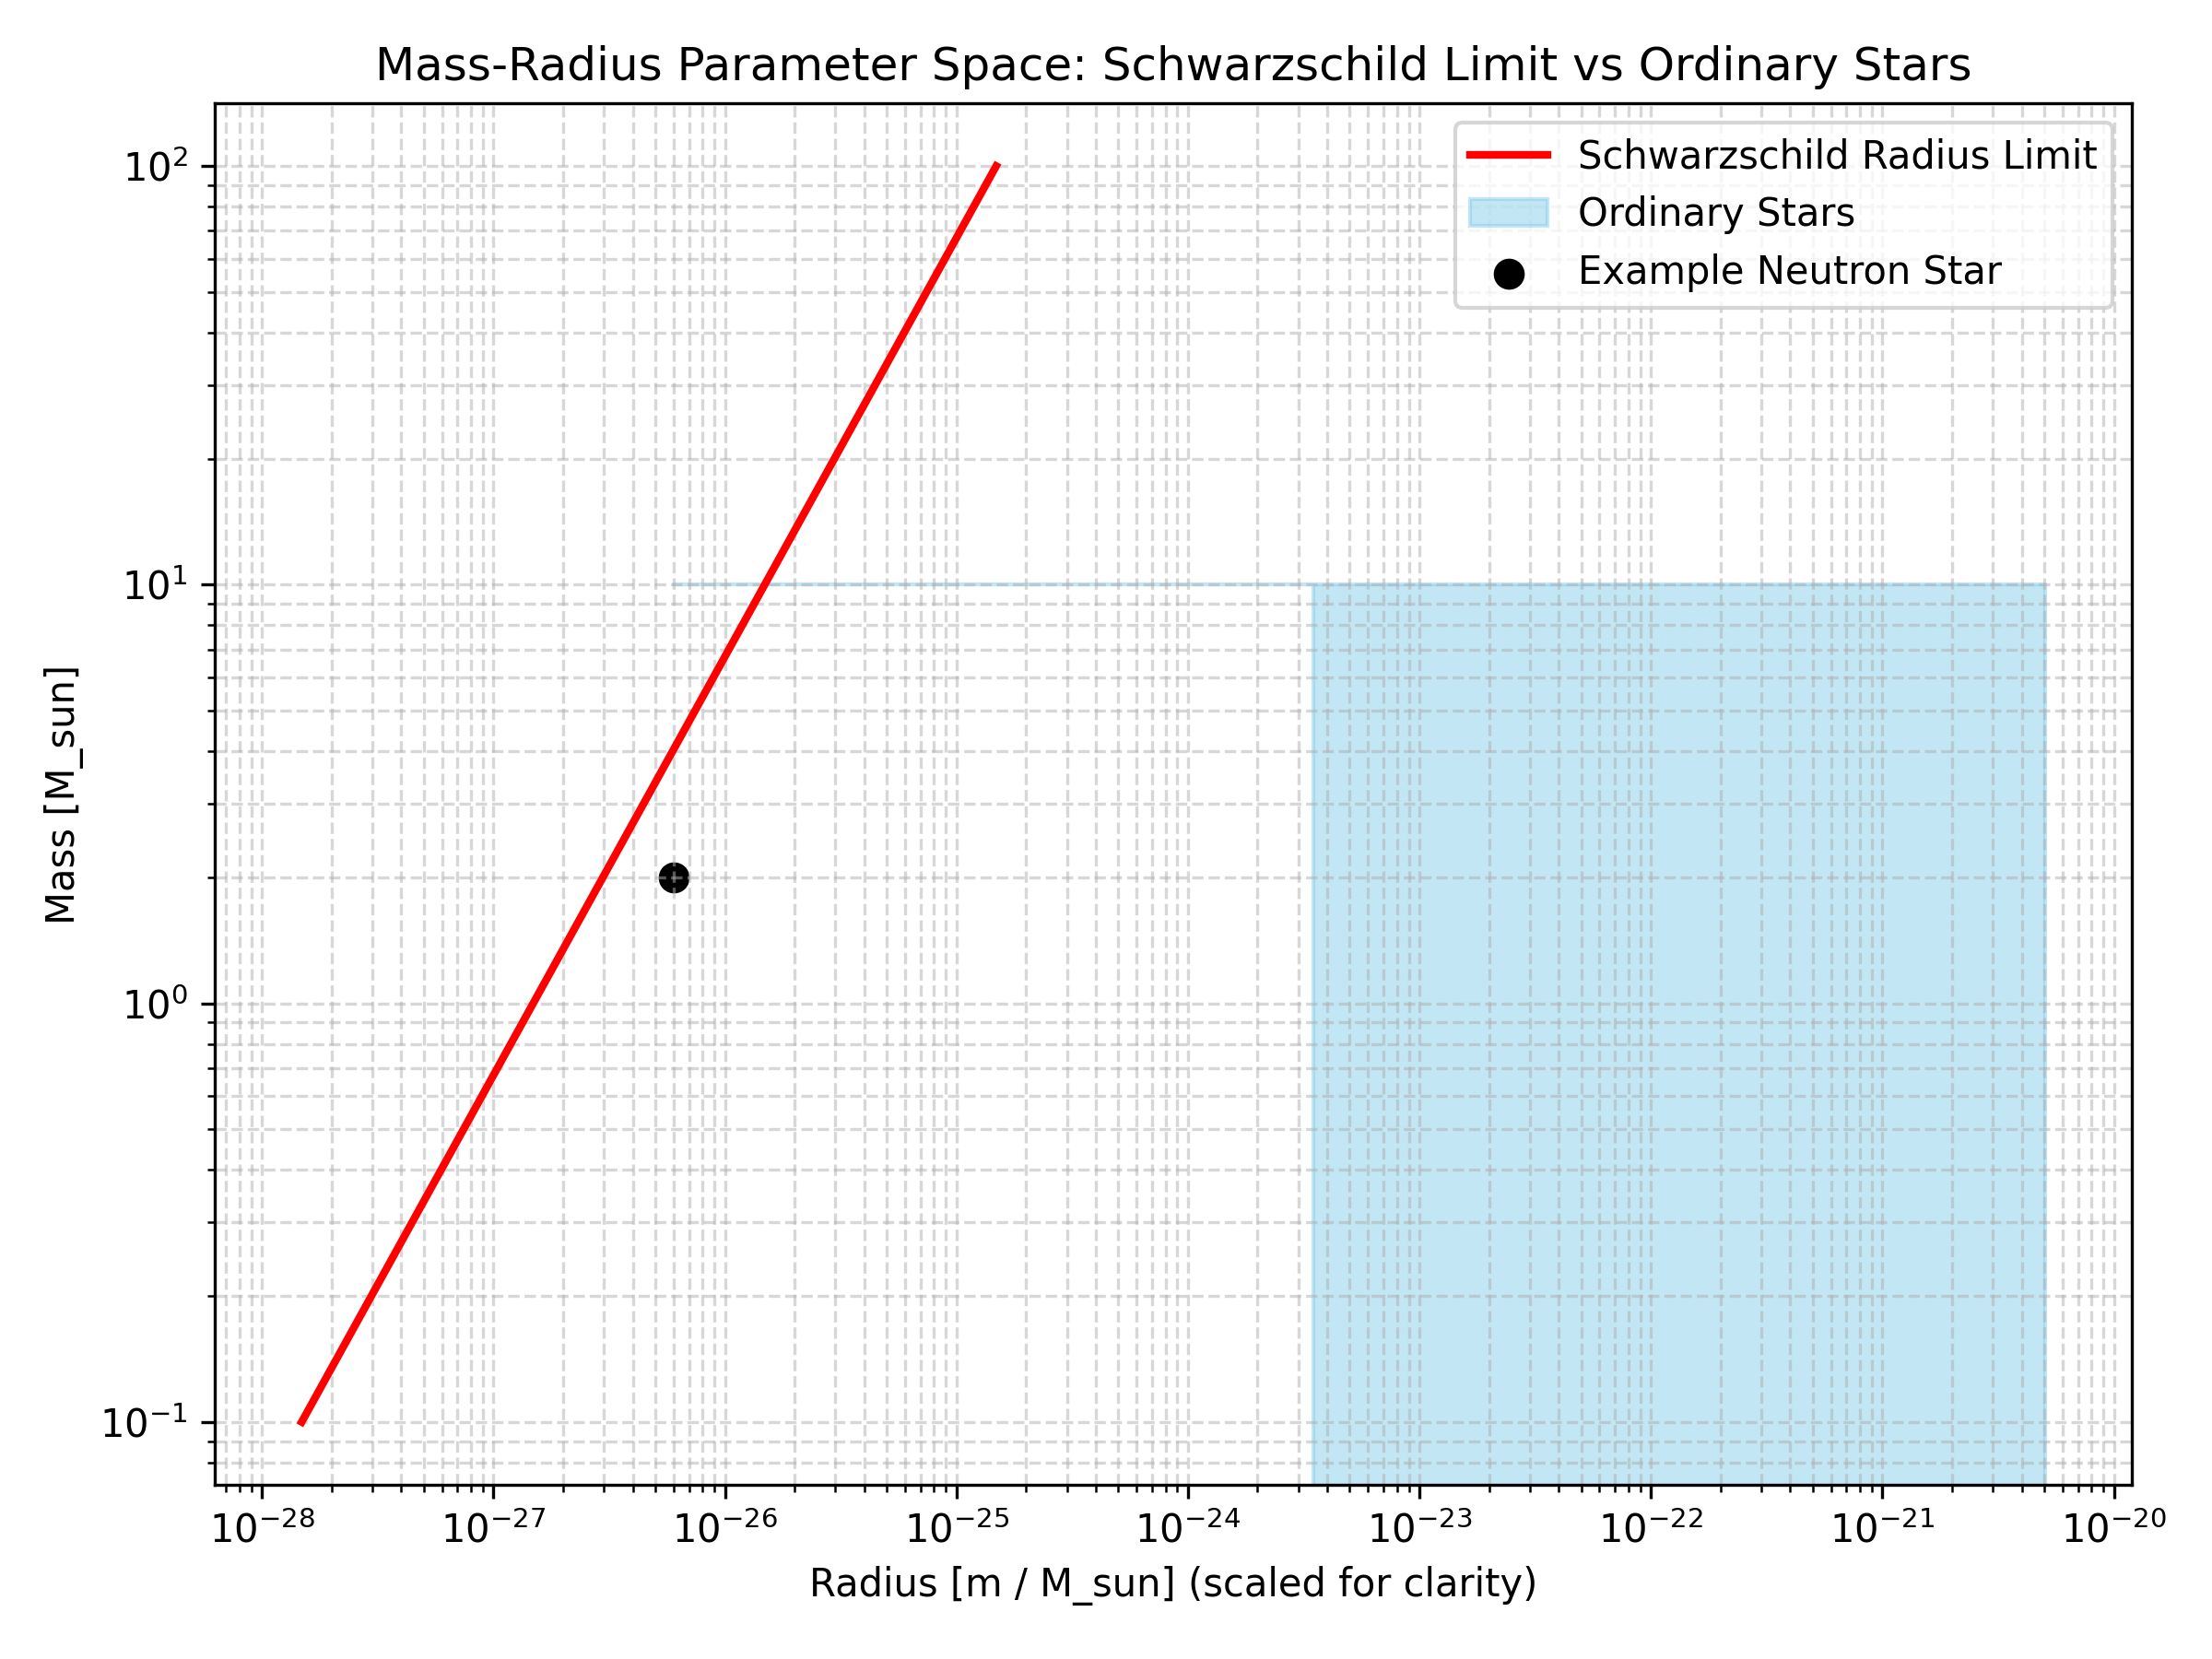
\includegraphics[width=0.7\textwidth]{figures/mass_radius_diagram.png}
    \caption{Mass--radius parameter space showing the Schwarzschild radius boundary (red line) marking the theoretical limit for black hole formation. Ordinary stars (blue region) lie safely below this limit, highlighting the gap between Newtonian intuition and relativistic reality.}\label{fig:mass-radius}
\end{figure}

By contrasting Newtonian approximations with calculus-based and relativistically informed analyses, this study systematically explores the mass\textendash{}radius parameter space of non-collapsed cosmic objects. Computational methods, including numerical evaluation of compactness and visualization of parameter regimes, are employed to distinguish physically meaningful results from misleading interpretations.

\section{A Naive but Misleading Schwarzschild Reformulation}

\subsection{Algebraic Reformulation}

The Schwarzschild radius is defined by the condition
\begin{equation}
\frac{2GM}{R} = c^2,
\end{equation}
which may be rearranged as
\begin{equation}
2GM = c^2 R.
\end{equation}

Introducing a formal kinematic interpretation, we write one factor of the speed of light as a ratio of differentials,
\begin{equation}
c = \frac{dx}{dt},
\end{equation}
while retaining the second factor explicitly. Substituting into the previous expression yields
\begin{equation}
2GM = c R \frac{dx}{dt}.
\end{equation}

Multiplying both sides by $dt$, we obtain
\begin{equation}
2GM\, dt = c R\, dx.
\label{eq:naive-differential}
\end{equation}

\subsection{Hypothetical Photon-Transit Interpretation and Black Hole Hypothesis}

Equation~\eqref{eq:naive-differential} can be interpreted under a formal but physically naive hypothesis. 
Let $x$ denote the total coordinate distance traversed by a photon along a straight radial path. 
Points $A$ and $B$ denote the start and end of the path, respectively, while $O$ marks the entry point of a black hole. 
Inside the event horizon ($x \ge O$), the physics is unknown and potentially dominated by extreme tidal forces and spaghettification, which stretch objects along the radial direction.

For simplicity, we assume a symmetric division of the trajectory such that
\[ OA = OB = \frac{x}{2}. \]

\begin{figure}[ht!]
    \centering
    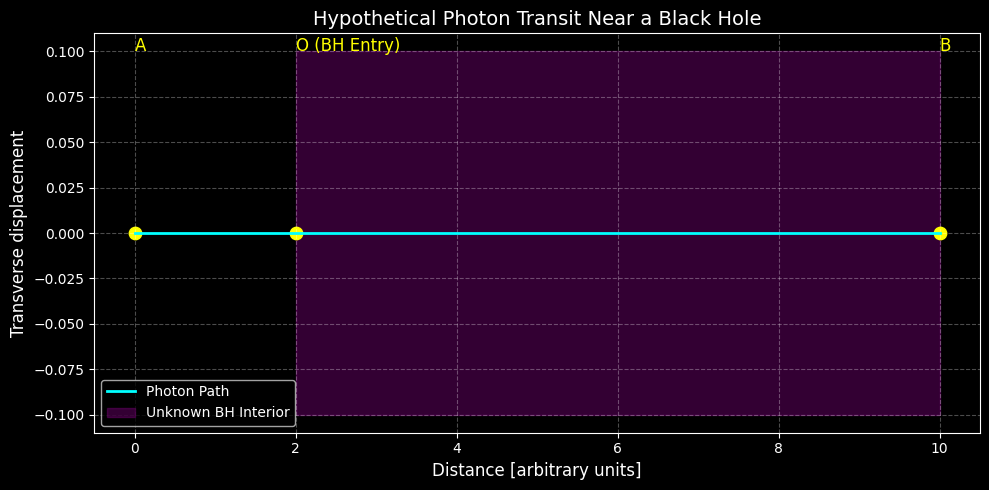
\includegraphics[width=0.8\textwidth]{figures/photon_bh_trajectory.png}
    \caption{Hypothetical photon trajectory near a black hole. The cyan line represents the photon path. The purple shaded region marks the black hole interior where physics is unknown, potentially dominated by spaghettification. O is the entry point of the black hole. This figure was generated programmatically using Python and Matplotlib. Minor computational steps involved Plotly and Manim for related illustrations.}\label{fig:photon-bh}
\end{figure}

\subsection{Formal Integration and Resulting Timescale}

Integrating both sides of Equation~\eqref{eq:naive-differential}, we write
\begin{equation}
\int_{0}^{T} 2GM \, dt = \int_{x/2}^{x} c R \, dx.
\end{equation}
The choice of integration limits reflects the assumptions made in this naive construction. 
On the left-hand side, we integrate over $t$ from $0$ to $T$, corresponding to the photon being emitted at point $A$ and reaching point $B$ along the trajectory. 
On the right-hand side, we integrate over $x$ from $x/2$ to $x$, reflecting the symmetric division of the path around the entry point $O$ of the black hole. 
This implicitly assumes that the photon travels along a straight radial line at constant speed $c$, both outside and (naively) inside the event horizon. 
While this choice is mathematically convenient, it does not correspond to any physically valid trajectory in general relativity, where spacetime curvature and tidal effects dominate.

Evaluating the integrals gives
\begin{equation}
2GM\, T = c R \left( x - \frac{x}{2} \right) = \frac{c R x}{2},
\end{equation}
which can be rearranged to
\begin{equation}
4GM\, T = c R x.
\end{equation}

While this derivation is mathematically consistent, it is physically naive: it ignores relativistic effects, the curvature of spacetime, and the impossibility of classical photon trajectories inside the event horizon. Therefore, despite its formal correctness, the result does not describe real black hole physics.
\subsection{Relativistic Characteristic Timescale}

While the preceding derivation is intentionally naive and does not represent
physically valid black hole dynamics, it nevertheless motivates a comparison
with timescales that are routinely employed in relativistic astrophysics.
In professional treatments of black holes, it is common to identify
\emph{characteristic scales} that set the natural units of length and time
for strong gravitational fields.

The most fundamental of these is the gravitational (or Schwarzschild) radius,
\[
r_g = \frac{2GM}{c^2},
\]
which emerges directly from the Schwarzschild solution of Einstein's field
equations. Rather than interpreting this quantity through escape velocity
arguments, modern treatments regard it as a geometric scale associated with
the causal structure of spacetime near a compact object~\cite{bambi2017, carlip2004}.

From this length scale, a corresponding characteristic timescale is obtained
by dividing by the speed of light,
\[
\tau = \frac{r_g}{c} = \frac{2GM}{c^3}.
\]
This timescale represents the order of magnitude of the time required for
light to traverse a region of spacetime comparable in size to the gravitational
radius. It therefore sets the fastest meaningful dynamical timescale for
processes occurring in the vicinity of a black hole, including horizon-scale
phenomena and strong-field relativistic effects~\cite{thorne1986, bambi2017}.

To illustrate its magnitude, consider a stellar-mass black hole with mass
$M = 10 M_\odot$. Substituting numerical values yields
\[
\tau \approx 5 \times 10^{-5}\,\text{s},
\]
or approximately $50\,\mu\text{s}$. For a supermassive black hole with
$M \sim 10^9 M_\odot$, the same expression gives a characteristic timescale of
order one hour. The linear dependence of $\tau$ on mass highlights the dramatic
separation of timescales between stellar-mass and supermassive black holes.

To emphasize this mass dependence, consider also an intermediate-mass black hole with $M \sim 10^4 M_\odot$:
\[
\tau \approx 5 \times 10^{-1}\,\text{s} = 0.5\,\text{s},
\]
showing how the timescale increases linearly with mass. Even a neutron-star-mass object ($M \sim 2 M_\odot$) would give $\tau \approx 10\,\mu\text{s}$, though it would not actually form a black hole.

The timescale $T$ obtained from our naive integration in Section~2.3, despite being derived from a Newtonian-inspired and physically inconsistent framework, is dimensionally comparable to this relativistic characteristic timescale $\tau$. This comparison is instructive: it demonstrates that even simple manipulations of the Schwarzschild condition can accidentally reproduce the correct \emph{order of magnitude} for characteristic timescales in black hole physics.

For the remainder of this analysis, we formally denote the timescale $T$ as $\Lambda$ (capital Lambda), the Integrated Traversal Time, which we shall now study in detail. This rebranding allows us to distinguish the heuristic construction from the rigorous relativistic results, while tracking how these two quantities compare across different mass and distance scales.

\section{Integrated Traversal Time}

The Integrated Traversal Time $\Lambda$ constitutes a fundamental quantity arising from the naive kinematic integration presented in Section~2.3. While this framework is heuristic in nature—neglecting gravitational redshift, coordinate singularities, and genuine horizon dynamics—it provides a structured and interpretable measure of path-dependent traversal durations within the simplified model. By dedicating a separate section to its development, we establish both its mathematical foundations and its relationship to the relativistic characteristic timescale $\tau$.

The development of $\Lambda$ distinguishes the heuristic, kinematic timescale constructed from flat-space Newtonian assumptions from the relativistic, geometrically meaningful timescale $\tau$ that emerges from general relativity. Despite their different conceptual origins, both timescales share the same dimensional structure and mass dependence. This symbolic distinction allows us to track how these two quantities compare across different regimes without conflating their physical interpretations.

\subsection{Formulation of the Integrated Traversal Time}

Starting from the integration of Section~2.3, we have
\begin{equation}
    4GM \, T = c \, R \, x,
\end{equation}
where $x$ denotes the radial coordinate interval traversed, and $R$ is the characteristic radius introduced in the model. Substituting the Schwarzschild radius $R = 2GM/c^2$ yields
\begin{equation}
    4GM \, T = c \left(\frac{2GM}{c^2}\right) x = \frac{2GM}{c} x.
\end{equation}

Dividing both sides by $4GM$ isolates the traversal timescale:
\begin{equation}
    T = \frac{x}{2c}.
\end{equation}

We now formally redefine this quantity as
\begin{equation}
    \Lambda \equiv T = \frac{x}{2c},
\end{equation}
the Integrated Traversal Time. The key observations underlying this expression are:

\begin{itemize}
    \item \textbf{Geometric origin:} The factor $x/2$ arises naturally from the symmetric geometric integration over the chosen radial interval in Section~2.3.
    \item \textbf{Kinematic approximation:} The speed of light $c$ is treated as constant, consistent with the flat-space kinematic framework employed throughout the heuristic construction.
    \item \textbf{Mass independence:} The mass parameter $M$ cancels entirely during the algebraic simplification, indicating that $\Lambda$ is a purely kinematic quantity that depends neither on gravitational dynamics nor on the properties of the source. This stands in sharp contrast to $\tau = 2GM/c^3$, which scales linearly with mass.
\end{itemize}

\subsection{Horizon-Scale Comparison: The Convergence of \texorpdfstring{$\Lambda$ and $\tau$}{Lambda and tau}}

The goal of this section is to demonstrate a numerical convergence between a heuristic kinematic model and General Relativity through high-school level algebra and dimensional analysis.

\subsubsection{Define \texorpdfstring{$\tau$}{tau}: The Relativistic Characteristic Timescale}

In General Relativity, black holes are characterized by a critical length scale known as the Schwarzschild radius:
\begin{equation}
    r_g = \frac{2GM}{c^2}
\end{equation}
where $G$ is the gravitational constant, $M$ is the mass, and $c$ is the speed of light. From this geometric scale, we derive a fundamental timescale representing the time required for light to traverse the Schwarzschild radius:
\begin{equation}
    \tau = \frac{r_g}{c}
\end{equation}

Substituting the expression for $r_g$, we obtain:
\begin{equation}
    \tau = \frac{2GM}{c^3}
\end{equation}

This quantity $\tau$ serves as the characteristic timescale of the black hole, setting the physical scale for the fastest possible processes near the event horizon.

\subsubsection{Define \texorpdfstring{$\Lambda$}{Lambda}: The Integrated Traversal Time}

From our earlier development in Section~3.1, we derived the Integrated Traversal Time as the time required for light to traverse a specified distance $x$ at constant speed $c$:
\begin{equation}
    \Lambda = \frac{x}{2c}
\end{equation}

This expression arises purely from kinematic considerations in the heuristic model and contains no gravitational mass dependence.

\subsubsection{Substitution \& Proof: Showing Convergence at the Horizon Scale}

To compare $\Lambda$ and $\tau$ directly, we now set the traversal distance $x$ equal to the diameter of the black hole event horizon:
\begin{center}
    $x = 2r_g$
\end{center}

Substituting this into the expression for $\Lambda$:
\begin{equation}
    \Lambda = \frac{2r_g}{2c}
\end{equation}

The factors of 2 in the numerator and denominator cancel, leaving:
\begin{equation}
    \Lambda = \frac{r_g}{c}
\end{equation}

But we defined $\tau = \frac{r_g}{c}$ above. Therefore, by simple algebraic cancellation, we have proven:
\begin{equation}
    \Lambda = \tau \quad \text{at the horizon scale}
\end{equation}

\subsubsection{Pedagogical Goal: Understanding Dimensional Analysis}

This proof illustrates a powerful principle: even when working with simplified, non-relativistic models, dimensional analysis and geometric reasoning can lead to correct characteristic scales. The convergence of $\Lambda$ and $\tau$ demonstrates that:

\begin{enumerate}
    \item \textbf{Dimensional consistency matters.} Both timescales have the dimension of time and involve the fundamental constant $c$. When dimensions are correct, the model captures the right order of magnitude.
    
    \item \textbf{Geometry provides natural scales.} The Schwarzschild radius $r_g$ emerges both in General Relativity and as a natural length scale in the heuristic model. This geometric role transcends the physical differences between the two approaches.
    
    \item \textbf{Algebra can be more transparent than calculus.} This proof uses only high-school level algebra—factoring, cancellation, and substitution—yet achieves a profound result: it shows that a heuristic model can predict the correct timescale at the horizon. Advanced calculus notation (like evaluation bars or integral limits) is unnecessary; simple substitution suffices.
    
    \item \textbf{Numerical agreement does not imply physical equivalence.} While $\Lambda = \tau$ at $x = 2r_g$, the two quantities have fundamentally different origins. $\tau$ emerges from General Relativity's description of curved spacetime; $\Lambda$ arises from flat-space kinematics. Their agreement at the horizon scale is a consequence of dimensional structure, not physical identity.
\end{enumerate}

This framework highlights how dimensional analysis serves as a bridge between simple models and sophisticated theories, enabling even elementary constructs to capture essential features of complex phenomena.
\subsection{Scaling Across Mass Regimes}

To illustrate the behavior of $\Lambda$ and $\tau$ across the full spectrum of black hole masses, Table~\ref{table:timescales} compares the two timescales at horizon-scale distances ($x = 2r_g$).

\begin{table}[h!]
\centering
\begin{tabular}{|c|c|c|c|}
\hline
\textbf{Black Hole Type} & \textbf{Mass ($M$)} & \textbf{Relativistic $\tau$} & \textbf{Integrated $\Lambda$ ($x = 2r_g$)} \\
\hline
Stellar-mass & $10\,M_\odot$ & $\sim 50\,\mu\text{s}$ & $\sim 50\,\mu\text{s}$ \\
Intermediate-mass & $10^4\,M_\odot$ & $\sim 0.05\,\text{s}$ & $\sim 0.05\,\text{s}$ \\
Supermassive & $10^9\,M_\odot$ & $\sim 1.5\,\text{hours}$ & $\sim 1.5\,\text{hours}$ \\
\hline
\end{tabular}
\caption{Comparison of the relativistic characteristic timescale $\tau$ and the integrated traversal time $\Lambda$ evaluated at horizon-scale distances ($x = 2r_g$).}
\label{table:timescales}
\end{table}

The table reveals a crucial distinction: when $x$ is fixed at horizon-scale (mass-dependent), both timescales display identical linear scaling with mass, mediated through $r_g$. However, for arbitrary traversal distances $x$ independent of the source mass, $\Lambda = x/(2c)$ exhibits no mass dependence whatsoever. This contrast reflects the kinematic essence of $\Lambda$ and underscores its origin in geometric constructs rather than genuine gravitational dynamics.

\subsection{Refined Interpretation}

The Integrated Traversal Time $\Lambda$ represents a dimensionally consistent and structurally coherent timescale arising from geometric considerations and kinematic assumptions within the simplified framework of Section~2.3. Its numerical agreement with the relativistic timescale $\tau$ at horizon-scale distances is noteworthy and instructive, yet it does not signify that $\Lambda$ captures genuine relativistic horizon-scale dynamics. Rather, $\Lambda$ serves as a clean, interpretable reference measure for path-dependent traversal durations, enabling direct comparison between heuristic kinematic models and fully relativistic formulations grounded in general relativity.

\subsubsection{Understanding the Distinction through Analogies}

To clarify why $\Lambda$ and $\tau$ can numerically agree while remaining conceptually distinct, consider the following everyday analogies:

\begin{enumerate}
    \item \textbf{The Ruler and the Road.} 
    Imagine measuring the distance a car travels on a straight road using a ruler. If the ruler is 30 cm long and the road is 30 km long, we can determine the travel time by dividing distance by speed: $t = 30\,\text{km} / 100\,\text{km/h} = 0.3\,\text{hours}$. This calculation is mathematically valid and gives the correct answer. However, the \emph{ruler itself} tells us nothing about how the car's engine works, the friction in the tires, or the road's condition. Similarly, $\Lambda = x/(2c)$ is a valid \emph{kinematic} measure of traversal duration that correctly relates distance to speed, but it carries no information about gravitational dynamics or spacetime curvature—phenomena captured by the truly relativistic quantity $\tau$.

    \item \textbf{The Menu and the Meal.} 
    A restaurant menu lists the names and prices of dishes in a way that is dimensionally consistent: each item has a price in dollars. One might calculate ``menu value per item'' and discover that, on average, each entry costs the same. This calculation is structurally sound, yet it tells us nothing about nutritional content, flavor, or cooking technique—the \emph{physics} of the meal itself. Likewise, $\Lambda$ and $\tau$ both have the dimension of time and may accidentally produce the same numerical value at certain scales (like $x = 2r_g$), but this dimensional agreement does not mean they encode the same physical insight. $\tau$ reveals something deep about the causal structure of spacetime near a black hole; $\Lambda$ reveals only how long light takes to traverse a given distance in flat space.

    \item \textbf{The Shadow and the Object.} 
    On a sunny afternoon, a building casts a shadow on the ground. The shadow's length depends on the sun's angle and the building's height, and we can calculate it using simple geometry. The shadow may even have the same length as a nearby tree. Yet the shadow is not the building, nor does it reveal the building's internal structure, materials, or architectural purpose. Similarly, $\Lambda$ is a ``shadow'' or heuristic projection of the Schwarzschild scale onto the kinematic framework. It can numerically match $\tau$ (just as the shadow matches the tree's length), but it does not reflect the deep relativistic physics governing black hole horizons.
\end{enumerate}

\subsubsection{Reconciling Agreement and Distinction}

This framework highlights the subtle interplay between dimensional consistency, geometric structure, and physical interpretation. The formal agreement between $\Lambda$ and $\tau$ at $x = 2r_g$ demonstrates that even elementary constructs can accidentally reproduce the correct order of magnitude for characteristic scales in black hole physics, provided that the underlying constants and dimensional analysis are respected. However, such agreement must not be conflated with physical equivalence; the relativistic timescale $\tau$ remains the authoritative measure for horizon-scale and strong-field phenomena, while $\Lambda$ functions as a pedagogical and heuristic reference point.

In summary: $\Lambda$ is to $\tau$ what a map is to a territory. Both provide useful information, and they may even coincide numerically at certain points, but only the territory (relativistic physics) truly describes what is happening at the black hole horizon.




\bibliographystyle{plain}
\bibliography{references}

\end{document}
